For an introduction into classical complexity theory. Refer to the standard textbooks aaran und cpo.
Rely an \cite[]{}
\section{Parametrized Complexity}

Introduced by Downey and Fellows \cite{Downey1999a}, parametrized complexity extends the classical theory with a framework that allows a more finely-grained analysis of computational problems. The idea is to measure a problem in terms of input size and an additional parameter $k$. This parameter denotes, how difficult the problem is: A larger parameter means a harder problem instance. We say that a problem is \textit{Fixed-Parameter Tractable} (FPT) if problem instances of size $n$ can be solved in $f(n)n^{\mathcal{O}(1)}$ time for some function $f$ independent of $n$. 

\paragraph{Ways to cope with NP-hard problem} Usually 

\begin{center}
    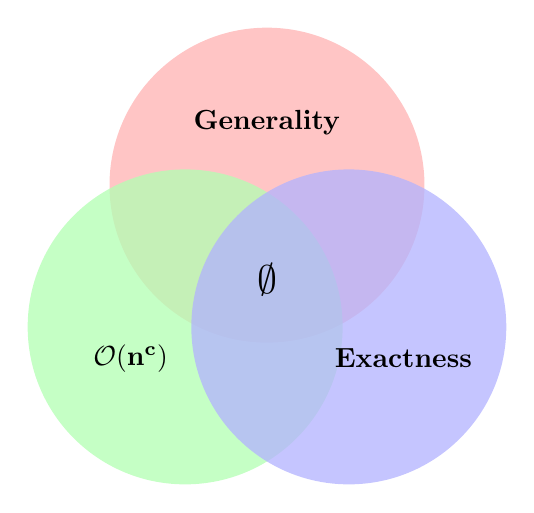
\begin{tikzpicture}
        \begin{scope}[blend mode = normal,opacity=0.75]
            \fill[red!30!white]   ( 90:1.2) circle (2);
            \fill[green!30!white] (210:1.2) circle (2);
            \fill[blue!30!white]  (330:1.2) circle (2);
        \end{scope}
        \node at ( 90:2)    {\textbf{Generality}};
        \node at ( 210:2)   {$\mathbf{\mathcal{O}(n^c)}$};
        \node at ( 330:2)   {\textbf{Exactness}};
        \node [font=\Large] {$\emptyset$};
    \end{tikzpicture}
\end{center}


\begin{definition}[Parametrized Problem{\cite[Def 1.1]{Cygan2015}}]
    A parametrized problem is a $L\subseteq\Sigma^*\times \mathbb{N}$ ($\Sigma$ finite fixed alphabet) for an instance $(x,k)\in \Sigma^*\times \mathbb{N}$, where k is called the \textit{parameter}.
\end{definition}

\begin{definition}[Instance Size]
    The \textbf{size of an instance} of an instance $(x,k)$ of a parametrized problem is $\abs{(x,k)} = \abs{x} + k$
\end{definition}
We will now clarify the basic terminology withing Parametrized Complexity. 
We are now giving a short introduction into the world of parametrized complexity. 
* General Introduction


\subsection{Fixed Parameter Tractability}

\begin{definition} [The Class FPT {\cite[Def 1.2]{Cygan2015}}]
    A parametrized problem $L\subseteq\Sigma^*\times\mathbb{N}$ is called \textit{fixed-parameter tractable} if there exists an algorithm A (called a \textit{fixed-parameter algorithm}), a computable function $f:\mathbb{N} \rightarrow \mathbb{N}$ and a constant c such that, given $(x,k) \in \Sigma^* \times \mathbb{N}$, the algorithm $\mathcal{A}$ correctly decides whether $(x,k) \in L$ in time bounded by $f(k) \cdot |(x,k)|^c$. The complexity class containing all fixed-parameter tractable problems is called \textit{FPT}
\end{definition}


\subsection{Kernelization}

\begin{definition}[kernelization Algoritm{\cite[Def 2.1]{Cygan2015}}]
A \textit{Kernelization Algorithm} or \textit{kernel} is an algorithm $\mathfrak{A}$ for a parametrized Problem Q, that given an instance $(I,k)$ of Q works in polynomial time and returns an equivalent instance $(I', k')$ of Q. Moreover, we require that $size_{\mathfrak{A}}(k) \leq g(k)$ for some computable function $g:\mathbb{N} \rightarrow \mathbb{N}$
\end{definition}

%TODO better
If we bound the size of the kernel by linear function $f(m) = \mathcal{O}(k)$, we say that the problem admits a \textbf{linear kernel}. 

%Examplary, if we reduce a graph for a graph problem in such a way that we can garuantee that our reduced graph only has a a few vertices \textbf{linear} in  $k$ left

The main idea, preprocessing algorithm, shrink size as much as possible, sound reduction rules,small output instance

\begin{definition}[Output size of a Preprocessing Procedure {\cite[p. 18]{Cygan2015}}] The output size of a preprocessing algorithms $\mathfrak{A}$ is defined as 

    \[\mathrm{size}_{\mathfrak{A}}(k) = \sup\{\abs{I'} + l': (I',k')= \mathfrak{A}(I,k), I \in \Sigma^* \} \]
\end{definition}

possibly infinite

Clearly, if there exists a kernelization algorithm for a problem $L$ and an algorithm $\mathfrak{A}$ with any runtime to decide $L$, the problem is in $FPT$ because after the kernelization pre-processing has been applied, the size of the reduced instance is a function merely in $k$ and independent of the input size $n$. In \cref{ch:linkern} we will explicitly construct a kernel for \psdom and hence showing it to be in \textit{FPT}. 

% Interstingly, als the converse?

\begin{definition}[Reduction Rules {\cite[p. 18]{Cygan2015}}]
A \textbf{reduction rule} is a function $\phi:\Sigma^* \times \mathbb{N} \rightarrow \Sigma^* \times \mathbb{N}$ that maps an instance $(x,k)$ to an equivalent instance $(x',k')$ such that $phi$ is computable in time polynomial in $\abs{x}$ and $k$
\end{definition}

\begin{definition}[Equivalent Instance {\cite[p. 18]{Cygan2015}}]
     This is a test
\end{definition}

\begin{definition}{Soundness of a rule}

\end{definition}

A \textbf{reduction rule} is a function $\Sigma* \times \mathbb{N}$ that maps an instance $(x,k)$ to an equivalent instance $(x',k')$ such that xx is computable in time polynomial in $\abs{x}$ and $k$

\subsection{Fixed Parameter Intractability: The w-Hierarchy}
\subsection{Compare to classical NP-Hardness theory}

\subsubsection{Parametrized Reductions}
\begin{definition}[Parametrized Reduction {\cite[Def 13.1]{Cygan2015}}] Let $A,B\subseteq \Sigma^*\times\mathbb{N}$ two parametrized problems. A \textit{Parametrized Reduction} from A to B is an algorithm that, given an instance $(x,k)$ of A, outputs an instance $(x', k')$ of B such that

    \begin{itemize}
        \item $(x,k)$ is a \textcolor{gray}{yes instance} of A \textbf{iff} $(x',k')$ is a \textcolor{gray}{yes instance} of B
        \item $k' \leq g(k)$ for some computable function $g$
        \item the running time is $f(k)\cdot |x|^{\mathcal{O}(1)}$ (FPT!)
    \end{itemize}
\end{definition}
    \subsubsection{The $w$-hierarchy}

